% Provenance (never printed): see sources/outline_sources.md (Year 3:
% stereographic projection; fold and fault analysis; palaeostress; balanced
% cross-sections). Brief: sources/book5/BRIEFS.md, ch. 8. Nets, pi-diagram and
% fault-slip data from figdata/bachelor-3/stereonet.py (Varden data invented,
% from figdata/shared/region.py); Fry plot from figdata/bachelor-3/fry.py.
% Exercise and problem values in the Book 5 scratch calculator calc/ch08.py.
% No real-world numbers: no ledger rows.
\chapter{Analisis Struktur}\label{ch:b3:structural-analysis}

Seorang geolog telah mengukur dua ratus bidang perlapisan pada sayap sebuah lipatan
terlalu besar untuk dilihat utuh: engselnya berada di bawah hutan, sayapnya membentang sepanjang
kilometer. Setiap pembacaan berupa sepasang bilangan. Diplot sebagai titik pada
bagan melingkar, \omterm{def:b3:structural-analysis:stereo}{kutub-kutub} bidang jatuh pada satu kurva, sebuah lingkaran besar, dan
\omterm{def:b3:structural-analysis:stereo}{kutub} lingkaran besar itu adalah sumbu lipatan, sebuah garis yang tidak seorang pun
pernah melihatnya. Bab ini membangun bagan, yaitu \omterm{def:b3:structural-analysis:stereo}{proyeksi stereografis}, dan
menggunakannya bersama alat-alat vektor di baliknya untuk mencari sumbu-sumbu lipatan, untuk mengukur
regangan yang terekam pada benda-benda terdeformasi, untuk memulihkan tegangan yang menggerakkan sekumpulan
sesar, dan untuk merestorasi penampang yang terdeformasi ke keadaan sebelum
deformasi.

\begin{recall}
Lingkaran besar dan kecil pada bola ada di volume Tahun 1, dalam babnya
tentang astronomi bola; jurus, kemiringan, arah kemiringan, tren, dan penunjaman
dibahas dalam bab-bab tentang peta geologi dan penampang;
normal satuan ke atas bidang dengan arah kemiringan $\alpha$ dan kemiringan $\delta$, $\vec n = (\sin\delta
\sin\alpha, \sin\delta\cos\alpha, \cos\delta)$ dalam komponen timur, utara, dan atas
dan rata-rata vektor dari sekumpulan pembacaan dalam bab pertamanya tentang
metode lapangan dan laboratorium. Unsur dan kelas lipatan, garis engsel suatu
lipatan sejajar dengan $\vec n_1\times\vec n_2$ dan sudut antar-sayap
$\ang{180} - \arccos(\vec n_1\cdot\vec n_2)$, serta teori Anderson tentang
pensesaran, dibahas dalam bab tentang sesar, lipatan, dan fabrik; tegangan,
tegangan utama, elips regangan, dan geser sederhana dalam bab tentang
tegangan, regangan, dan reologi; rake vektor gelincir (dari jurus,
\ang{-90} untuk sesar normal, \ang{90} untuk sesar naik, 0 sinistral dan
\ang{180} dekstral), dan sumbu P dan T dari mekanisme fokus dalam bab tentang
sumber gempa bumi. Penampang seimbang dan décollement dibahas dalam
volume Tahun 2, dalam bab tentang Alpen. Kuadrat terkecil dibahas dalam
\cref{sec:b3:seismology-imaging:inverse}; nilai eigen dan vektor eigen dari
matriks simetris dibahas dalam buku matematika.
\end{recall}

\section{Proyeksi stereografis}\label{sec:b3:structural-analysis:stereo}

Data geolog berupa orientasi: orientasi bidang perlapisan, sebuah
sesar, sebuah foliasi; tren dan penunjaman lineasi, engsel lipatan, arah
gelincir. Masing-masing adalah arah yang melalui sebuah titik, tanpa posisi. Untuk
membandingkan ratusan di antaranya, bayangkan semuanya dipindahkan ke pusat satu bola:
sebuah garis menembus belahan bawah bola di satu titik, sebuah bidang memotongnya sepanjang
setengah lingkaran besar. Bagan belahan bawah kemudian menampilkan garis sebagai
titik dan bidang sebagai kurva.

\begin{definition}[Proyeksi stereografis, jaring sama sudut, proyeksi sama luas, kutub]\label{def:b3:structural-analysis:stereo}
Misalkan sebuah garis melalui pusat $O$ bola berjari-jari $R$ memotong belahan bawah
di titik $P$, pada sudut $\theta = \ang{90} - p$ dari nadir, dengan $p$
adalah penunjaman garis dan $t$ trennya. Yang disebut \emph{proyeksi
stereografis}\index{proyeksi stereografis} memetakan $P$ ke titik tempat
garis lurus dari zenit ke $P$ memotong bidang horizontal melalui
$O$; titik itu berjarak $r$ dari $O$ pada azimut $t$.
Bagan belahan bawah yang digambar dengan cara ini, beserta kisinya berupa lingkaran besar dan
lingkaran kecil, adalah \emph{jaring sama sudut}\index{jaring sama sudut} (atau
jaring Wulff). Yang disebut \emph{proyeksi sama luas}\index{proyeksi sama luas}
memetakan $P$ ke titik yang berjarak $r =
R\sqrt2\sin(\theta/2)$ pada azimut $t$; jaringnya adalah jaring Schmidt.
Yang disebut \emph{kutub}\index{kutub (ke bidang)} sebuah bidang adalah garis normalnya, yang diplot
sebagai titik: untuk bidang dengan arah kemiringan $\alpha$ dan kemiringan $\delta$, kutubnya
memiliki tren $\alpha + \ang{180}$ dan penunjaman $\ang{90} - \delta$.
\end{definition}

Kedua proyeksi menempatkan garis vertikal di pusat dan garis horizontal pada
lingkaran berjari-jari $R$, yaitu primitif. Keduanya berbeda dalam hal yang dipertahankan.

\begin{theorem}[Kedua proyeksi]\label{thm:b3:structural-analysis:projections}
\begin{enumerate}[label=(\alph*)]
  \item \omterm{def:b3:structural-analysis:stereo}{Proyeksi stereografis} menempatkan $P$ pada $r = R\tan(\theta/2)$. Ia
        bersifat konform: di setiap titik semua arah diregangkan dengan
        faktor yang sama, $1/(2\cos^2(\theta/2))$, sehingga sudut antara
        kurva tetap terjaga.
  \item \omterm{def:b3:structural-analysis:stereo}{Proyeksi sama luas} mengalikan setiap luas dengan faktor yang sama,
        $1/2$: luas suatu wilayah pada jaring adalah setengah luas
        wilayah belahan bola yang diwakilinya.
\end{enumerate}
\end{theorem}

\begin{proof}
(a) Pada bidang vertikal yang melalui zenit $Z$, nadir, dan $P$
(gambar pertama di bawah), busur dari nadir ke $P$
menghadap sudut $\theta$ di pusat, sehingga sudut keliling
$\theta/2$ di $Z$, yang berjarak $R$ di atas $O$: $r =
R\tan(\theta/2)$. Langkah kecil $R\,\mathrm d\theta$ pada bola menuju
nadir menjadi $\mathrm dr = R\,\mathrm d\theta/(2\cos^2(\theta/2))$ pada
bagan. Lingkaran titik-titik pada sudut $\theta$ dari nadir memiliki
keliling $2\pi R\sin\theta$ dan menjadi lingkaran dengan keliling $2\pi
r$; rasionya adalah $\tan(\theta/2)/\sin\theta = 1/(2\cos^2(\theta/2))$, sama
seperti sepanjang jari-jari. Peta yang meregang sama di dua arah tegak lurus
meregang sama ke segala arah dan mempertahankan sudut.

(b) Tudung bola dalam sudut $\theta$ dari nadir memiliki luas
$2\pi R^2(1 - \cos\theta) = 4\pi R^2\sin^2(\theta/2)$; bayangannya adalah cakram
dengan luas $\pi r^2 = 2\pi R^2\sin^2(\theta/2)$, setengahnya. Kedua luas
dibagi rata menurut azimut, sehingga sektor tudung antara dua azimut
dan bayangannya mempertahankan rasio $1/2$, begitu pula cincin antara dua nilai
$\theta$, yaitu selisih dua tudung. Setiap wilayah adalah gabungan sektor-sektor
cincin kecil semacam itu.
\end{proof}

\omterm{def:b3:structural-analysis:stereo}{Proyeksi stereografis} juga memetakan setiap lingkaran pada bola, besar maupun
kecil, menjadi lingkaran atau garis lurus pada bagan; hal ini kita terima tanpa bukti. Hal itu membuat
\omterm{def:b3:structural-analysis:stereo}{jaring sama sudut} mudah digambar dengan jangka, dan lingkaran kecil, yaitu kerucut
garis-garis pada sudut tetap dari suatu sumbu, mempertahankan bentuknya. \omterm{def:b3:structural-analysis:stereo}{Proyeksi sama
luas} mendistorsi bentuk: lingkaran kecil menjadi oval yang terentang
mengelilingi primitif. Itulah proyeksi tempat awan \omterm{def:b3:structural-analysis:stereo}{kutub} dapat
dihitung, karena luas yang sama pada jaring memuat bagian yang sama dari
arah belahan bola; geolog struktur, dan seismolog untuk
mekanisme fokus mereka, menggunakannya untuk data mereka.

\begin{omfigure}
\begin{tikzpicture}[scale=1.0, >=stealth]
% (a) equal-angle: theta = 60 deg, R = 2 cm; r = 2 tan 30 = 1.155
\begin{scope}
\draw[thick] (0,0) circle (2);
\draw (-2.5,0) -- (2.5,0) node[right, font=\scriptsize] {bidang};
\fill (0,2) circle (1.5pt) node[above, font=\scriptsize] {zenit $Z$};
\fill (0,-2) circle (1.5pt) node[below, font=\scriptsize] {nadir};
\fill (0,0) circle (1.2pt) node[above left, font=\scriptsize] {$O$};
\draw[dashed] (0,2) -- (0,-2);
\draw[omDef, thick] (0,0) -- (1.732,-1);
\fill[omDef] (1.732,-1) circle (1.5pt) node[below right, font=\scriptsize] {$P$};
\draw[omThm] (0,2) -- (1.732,-1);
\fill[omThm] (1.155,0) circle (1.5pt);
\node[omThm, font=\scriptsize, above right] at (1.155,0) {$P'$};
\draw (0,-0.6) arc[start angle=-90, end angle=-30, radius=0.6];
\node[font=\scriptsize] at (0.38,-0.85) {$\theta$};
\draw (0,1.2) arc[start angle=-90, end angle=-60, radius=0.8];
\node[font=\scriptsize] at (0.25,0.95) {$\theta/2$};
\draw[<->] (0,0.25) -- (1.155,0.25);
\node[font=\scriptsize, above] at (0.58,0.25) {$r$};
\node[font=\small] at (0,-3.0) {(a) sama sudut};
\end{scope}
% (b) equal-area: chord from nadir to P = 2R sin(theta/2) = 2
\begin{scope}[xshift=6.6cm]
\draw[thick] (0,0) circle (2);
\draw (-2.5,0) -- (2.5,0);
\draw (-2.5,-2) -- (2.5,-2) node[right, font=\scriptsize] {bidang singgung};
\fill (0,-2) circle (1.5pt) node[below left, font=\scriptsize] {nadir};
\fill (0,0) circle (1.2pt) node[above left, font=\scriptsize] {$O$};
\draw[dashed] (0,2) -- (0,-2);
\draw[omDef, thick] (0,0) -- (1.732,-1);
\fill[omDef] (1.732,-1) circle (1.5pt) node[above right, font=\scriptsize] {$P$};
\draw[omThm] (0,-2) -- (1.732,-1);
\draw[omThm, dashed] (1.732,-1) arc[start angle=30, end angle=0, radius=2];
\fill[omThm] (2,-2) circle (1.5pt);
\node[omThm, font=\scriptsize, below] at (2,-2.05) {$2R\sin(\theta/2)$};
\draw (0,-0.6) arc[start angle=-90, end angle=-30, radius=0.6];
\node[font=\scriptsize] at (0.38,-0.85) {$\theta$};
\node[font=\small] at (0,-3.0) {(b) sama luas};
\end{scope}
\end{tikzpicture}

\par\smallskip{\small Kedua proyeksi, pada bidang vertikal melalui garis
$OP$. (a) \omterm{def:b3:structural-analysis:stereo}{Proyeksi stereografis} memetakan $P$ ke $P'$, yaitu titik tempat garis
dari zenit memotong bidang horizontal: sudut di $Z$ adalah
$\theta/2$, sehingga $r = R\tan(\theta/2)$. (b) \omterm{def:b3:structural-analysis:stereo}{Proyeksi sama luas} memindahkan
$P$, di sekitar nadir, ke bidang singgung pada jarak $2R\sin(\theta/2)$
dari tali busur; bagan kemudian diskalakan dengan $1/\sqrt2$ sehingga garis-garis
horizontal jatuh pada primitif berjari-jari $R$.}\label{fig:b3:structural-analysis:geometry}
\end{omfigure}

\begin{omfigure}
\begin{tikzpicture}
\begin{groupplot}[group style={group size=2 by 1, horizontal sep=0.8cm},
  width=0.5\linewidth, height=0.5\linewidth, axis equal image, hide axis,
  xmin=-1.15, xmax=1.15, ymin=-1.15, ymax=1.15, unbounded coords=jump,
  title style={font=\small}]
\nextgroupplot[title={(a) jaring sama sudut (Wulff)}]
% computed in figdata/bachelor-3/stereonet.py
\addplot[gray!75, very thin] table[x=x, y=y] {figdata/out/bachelor-3-stereonet-wulff.dat};
\addplot[gray!75, very thin] coordinates {(-1,0) (1,0)};
\addplot[black, thick, domain=0:360, samples=181] ({cos(x)}, {sin(x)});
\node[font=\scriptsize, above] at (axis cs:0,1.0) {U};
\nextgroupplot[title={(b) jaring sama luas (Schmidt)}]
\addplot[gray!75, very thin] table[x=x, y=y] {figdata/out/bachelor-3-stereonet-schmidt.dat};
\addplot[gray!75, very thin] coordinates {(-1,0) (1,0)};
\addplot[black, thick, domain=0:360, samples=181] ({cos(x)}, {sin(x)});
\node[font=\scriptsize, above] at (axis cs:0,1.0) {U};
\end{groupplot}
\end{tikzpicture}

\par\smallskip{\small Kedua jaring, digambar dari rumus-rumus pada teorema
di atas: lingkaran besar dari bidang berjurus utara--selatan dan berkemiringan
\ang{10} ke timur dan ke barat, serta lingkaran kecil setiap \ang{10} terhadap
sumbu utara--selatan. Pada \omterm{def:b3:structural-analysis:stereo}{jaring sama sudut}, lingkaran kecil tetap berupa lingkaran;
pada jaring sama luas, lingkaran kecil berupa oval, tetapi luas yang sama memuat
bagian yang sama dari arah-arah.}\label{fig:b3:structural-analysis:nets}
\end{omfigure}

\paragraph{Bidang, garis dan sudut.}
Bidang dengan arah kemiringan $\alpha$ dan kemiringan $\delta$ memotong belahan bawah
sepanjang setengah lingkaran besar. Ujung-ujungnya terletak pada primitif di kedua ujung
jurus; titik tengahnya adalah garis kemiringan terbesar, yang menunjam $\delta$
ke arah $\alpha$; dan \omterm{def:b3:structural-analysis:stereo}{kutubnya} berjarak \ang{90} dari setiap titik padanya, pada
azimut $\alpha + \ang{180}$. Garis di dalam bidang adalah sebuah titik pada lingkaran besar.
Untuk memplot data, lembaran tembus pandang diletakkan di atas jaring dan diputar
terhadap pusat sampai jurus data berimpit dengan diameter utara--selatan jaring; lingkaran besar
dengan kemiringan yang tepat kemudian digambar, lalu lembaran diputar kembali.
Sudut antara dua garis diukur sepanjang lingkaran besar yang melalui kedua titik itu,
dengan menghitung pembagian lingkaran kecil yang dilintasinya, setelah lembaran
diputar sampai kedua titik terletak pada satu lingkaran besar pada jaring. Sudut antara
dua bidang adalah sudut antara \omterm{def:b3:structural-analysis:stereo}{kutub-kutubnya}, atau suplemennya.
Komputer melakukan hal yang sama dengan vektor: sudut antara dua garis dengan vektor satuan
$\vec u$ dan $\vec v$ adalah $\arccos|\vec u\cdot\vec v|$.

\begin{method}[Memutar data terhadap sumbu]\label{met:b3:structural-analysis:rotation}
Untuk membatalkan kemiringan, misalnya untuk mengembalikan lapisan ke posisi
horizontal bersama lineasi yang dibawanya, atau untuk memulihkan arah paleomagnetik yang
diukur pada strata miring (\cref{ch:b3:palaeomagnetism}):
\begin{enumerate}
  \item Pilih sumbu rotasi: untuk lapisan miring, garis jurusnya,
        yang horizontal; sudutnya adalah kemiringan, ke arah yang membawa lapisan naik.
  \item Pada jaring, putar lembaran sampai sumbu terletak di sepanjang
        diameter utara--selatan, tempat lingkaran-lingkaran kecil merupakan kerucut
        terhadap sumbu itu.
  \item Pindahkan setiap titik sepanjang lingkaran kecilnya sebesar sudut rotasi,
        diukur pada lingkaran-lingkaran besar. Titik yang akan keluar dari belahan bawah
        muncul kembali di ujung seberang lingkaran kecilnya,
        pada azimut yang berlawanan.
  \item Putar lembaran kembali. Dengan vektor, rotasi $\vec v$ sebesar
        sudut $\omega$ terhadap sumbu satuan $\vec k$ adalah $\vec v' = \vec v
        \cos\omega + (\vec k\times\vec v)\sin\omega + \vec k(\vec k\cdot\vec
        v)(1 - \cos\omega)$.
\end{enumerate}
\end{method}

\section{Analisis lipatan}\label{sec:b3:structural-analysis:folds}

Lipatan silindris dibentuk oleh sebuah garis lurus, yakni sumbu lipatan, yang digeser
sejajar dengan dirinya sendiri. Setiap bidang yang menyinggung permukaan terlipat memuat
sumbu itu, sehingga setiap normal terhadap permukaan tegak lurus pada sumbu: semua
\omterm{def:b3:structural-analysis:stereo}{kutub} terletak pada lingkaran besar dari bidang yang tegak lurus sumbu itu.

\begin{definition}[Diagram pi, sumbu beta]\label{def:b3:structural-analysis:pi}
Yang disebut \emph{diagram pi}\index{diagram pi} suatu lipatan adalah plot \omterm{def:b3:structural-analysis:stereo}{kutub-kutub}
bidang yang diukur pada permukaan terlipatnya. Untuk lipatan silindris, \omterm{def:b3:structural-analysis:stereo}{kutub-kutubnya} jatuh pada
sebuah lingkaran besar, yakni sabuk-$\pi$; \omterm{def:b3:structural-analysis:stereo}{kutub} sabuk itu ialah
\emph{sumbu beta}\index{sumbu beta}, taksiran sumbu lipatan yang diberikan oleh
pengukuran.
\end{definition}

Dengan dua sayap saja, \omterm{def:b3:structural-analysis:pi}{sumbu beta} adalah hasil kali silang normal-normalnya, seperti
yang ditunjukkan volume Tahun 1 untuk garis engsel. Dengan dua ratus pembacaan yang tersebar,
diperlukan kecocokan terbaik. Rata-rata vektor, yang berguna untuk pembacaan
satu bidang, tidak akan cukup: \omterm{def:b3:structural-analysis:stereo}{kutub-kutub} sabuk menunjuk ke segala arah sepanjangnya, dan
rata-ratanya sedikit mengatakan tentang lingkaran tempat \omterm{def:b3:structural-analysis:stereo}{kutub-kutub} itu berada.

\begin{definition}[Tensor orientasi]\label{def:b3:structural-analysis:orientation-tensor}
Yang disebut \emph{tensor orientasi}\index{tensor orientasi} dari $N$ vektor satuan
$\vec p_1, \dots, \vec p_N$ adalah matriks simetris
\[
  T = \frac1N\sum_{i=1}^N \vec p_i\,\vec p_i^{\mathsf T},
  \qquad T_{jk} = \frac1N\sum_i p_{ij}\,p_{ik} .
\]
Tensor ini tidak berubah jika sebuah vektor diganti dengan vektor kebalikannya, sehingga cocok untuk
sumbu dan \omterm{def:b3:structural-analysis:stereo}{kutub}, yang tidak memiliki arah. Nilai eigennya $\lambda_1 \ge \lambda_2
\ge \lambda_3 \ge 0$ berjumlah sama dengan jejaknya, yaitu $1$.
\end{definition}

\begin{theorem}[Gerombol dan sabuk dari tensor orientasi]\label{thm:b3:structural-analysis:tensor}
Untuk sembarang vektor satuan $\vec u$,
\[
  \frac1N\sum_{i=1}^N (\vec p_i\cdot\vec u)^2 = \vec u^{\mathsf T}T\,\vec u ,
\]
yang mencapai nilai terkecilnya, $\lambda_3$, saat $\vec u$ adalah vektor eigen
$\vec e_3$ dari nilai eigen terkecil, dan nilai terbesarnya, $\lambda_1$, sepanjang
vektor eigen $\vec e_1$. Karena $\vec p_i\cdot\vec u$ adalah sinus sudut
antara $\vec p_i$ dan bidang yang tegak lurus $\vec u$, lingkaran besar
yang tegak lurus $\vec e_3$ adalah sabuk yang meminimalkan jumlah kuadrat
sinus jarak \omterm{def:b3:structural-analysis:stereo}{kutub-kutub} ke lingkaran itu, dan $\sqrt{\lambda_3}$ adalah
akar rata-rata kuadrat sinusnya. Sumbu $\vec e_1$ adalah garis yang paling dekat dengan
vektor-vektor itu, yaitu sumbu rata-rata sebuah gerombol.
\end{theorem}

\begin{proof}
$(\vec p_i\cdot\vec u)^2 = \vec u^{\mathsf T}\vec p_i\,\vec p_i^{\mathsf T}\vec
u$; rata-ratakan atas $i$. Matriks $T$ simetris, sehingga memiliki basis ortonormal
dari vektor-vektor eigen, dengan $\vec u = \sum_k u_k\vec e_k$ dan $\sum_k
u_k^2 = 1$ dan $\vec u^{\mathsf T}T\vec u = \sum_k\lambda_k u_k^2$. Ini adalah
rata-rata berbobot dari nilai eigen, dengan bobot $u_k^2$ yang berjumlah 1: ia
terletak di antara $\lambda_3$ dan $\lambda_1$, dan mencapainya untuk $\vec u = \vec
e_3$ dan $\vec e_1$.
\end{proof}

Nilai-nilai eigen menggambarkan bentuk data. Gerombol memiliki $\lambda_1$ mendekati
1 dan dua lainnya kecil; sabuk memiliki $\lambda_3$ mendekati 0, dengan \omterm{def:b3:structural-analysis:stereo}{kutub-kutubnya}
tersebar sepanjang lingkaran sehingga $\lambda_1$ dan $\lambda_2$ membagi sisanya;
vektor yang tersebar merata memberikan tiga nilai eigen mendekati $1/3$. Suatu lipatan
silindris, dalam ketelitian pembacaan, jika $\sqrt{\lambda_3}$
tidak lebih besar daripada sebaran pembacaan berulang dari satu bidang. Lipatan kerucut,
atau dua generasi lipatan, menyebarkan \omterm{def:b3:structural-analysis:stereo}{kutub} menjauh dari lingkaran besar mana pun
dan menaikkan $\lambda_3$.

Gambar di bawah memplot dua belas pembacaan dari kedua sayap antiklin Varden
lipatan rekaan dalam seri ini (\cref{pb:b3:structural-analysis:1}
menghitung sumbunya). \omterm{def:b3:structural-analysis:stereo}{Kutub} dari sayap landai berkelompok dekat pusat
jaring dalam dua kelompok, yang bersama-sama mendefinisikan sabuk yang membentang hampir
timur--barat; \omterm{def:b3:structural-analysis:pi}{sumbu beta} terletak pada lingkaran primitif, hampir tepat ke utara. Bidang-bidang rata-rata
kedua sayap, yang digambar sebagai lingkaran besar, berpotongan di titik yang sama:
\omterm{def:b3:structural-analysis:pi}{sumbu beta} adalah garis yang dimiliki bersama oleh semua sayap.

\begin{omfigure}
\begin{tikzpicture}
\begin{groupplot}[group style={group size=2 by 1, horizontal sep=1.0cm},
  width=0.5\linewidth, height=0.5\linewidth, axis equal image,
  unbounded coords=jump, title style={font=\small}]
\nextgroupplot[hide axis, xmin=-1.15, xmax=1.15, ymin=-1.15, ymax=1.15,
  title={(a) belahan bawah}]
% computed in figdata/bachelor-3/stereonet.py (Varden readings invented)
\addplot[gray!35, very thin] table[x=x, y=y] {figdata/out/bachelor-3-stereonet-schmidt.dat};
\addplot[black, thick, domain=0:360, samples=181] ({cos(x)}, {sin(x)});
\addplot[gray, densely dashed] table[x=x, y=y] {figdata/out/bachelor-3-stereonet-limbs.dat};
\addplot[omDef, thick] table[x=x, y=y] {figdata/out/bachelor-3-stereonet-girdle.dat};
\addplot[only marks, mark=*, mark size=1.2pt] table[x=x, y=y] {figdata/out/bachelor-3-stereonet-poles.dat};
\addplot[only marks, mark=triangle*, mark size=3pt, omThm] table[x=x, y=y] {figdata/out/bachelor-3-stereonet-beta.dat};
\node[font=\scriptsize, above] at (axis cs:0,1.02) {U};
\node[omThm, font=\scriptsize, right] at (axis cs:0.06,0.88) {$\beta$};
\draw[gray] (axis cs:-0.3,-0.3) rectangle (axis cs:0.3,0.3);
\nextgroupplot[xmin=-0.3, xmax=0.3, ymin=-0.3, ymax=0.3, title={(b) pusat, diperbesar},
  xtick=\empty, ytick=\empty]
\addplot[gray!35, very thin] table[x=x, y=y] {figdata/out/bachelor-3-stereonet-schmidt.dat};
\addplot[omDef, thick] table[x=x, y=y] {figdata/out/bachelor-3-stereonet-girdle.dat};
\addplot[only marks, mark=*, mark size=1.5pt] table[x=x, y=y] {figdata/out/bachelor-3-stereonet-poles.dat};
\node[font=\scriptsize, align=center] at (axis cs:0.16,0.09) {kutub sayap\\ barat};
\node[font=\scriptsize, align=center] at (axis cs:-0.16,0.09) {kutub sayap\\ timur};
\node[omDef, font=\scriptsize] at (axis cs:0.17,-0.06) {sabuk-$\pi$};
\end{groupplot}
\end{tikzpicture}

\par\smallskip{\small \omterm{def:b3:structural-analysis:pi}{Diagram pi} antiklin Varden pada jaring sama luas,
belahan bawah: \omterm{def:b3:structural-analysis:stereo}{kutub} dari dua belas pembacaan perlapisan (titik),
sabuk kecocokan terbaik dari \omterm{def:b3:structural-analysis:orientation-tensor}{tensor orientasi} (biru), lingkaran besar dari
kedua sayap rata-rata (putus-putus) dan \omterm{def:b3:structural-analysis:pi}{sumbu beta} (segitiga), tempat ketiga lingkaran besar
bertemu. Lapisan yang miring ke timur memiliki \omterm{def:b3:structural-analysis:stereo}{kutub} di sebelah barat
dari pusat.}\label{fig:b3:structural-analysis:pi}
\end{omfigure}

\section{Analisis regangan berhingga}\label{sec:b3:structural-analysis:strain}

Batuan yang terdeformasi merekam regangannya ketika memuat objek yang bentuk asalnya
atau susunan asalnya diketahui: ooid bulat dan bintik reduksi,
fosil dengan simetri yang diketahui, kerakal, atau sekadar pusat-pusat butir
yang dahulu tersebar merata.

\begin{definition}[Analisis regangan berhingga, metode Fry]\label{def:b3:structural-analysis:strain-analysis}
Yang disebut \emph{analisis regangan berhingga}\index{analisis regangan berhingga} adalah pengukuran
elips regangan, atau elipsoid, yang dialami batuan, dari
bentuk, orientasi, atau jarak antarobjek yang keadaannya sebelum
deformasi diketahui. Dalam \emph{metode Fry}\index{metode Fry}, vektor
dari pusat setiap objek ke pusat setiap objek lainnya diplot dari
satu titik asal yang sama; ketika pusat-pusatnya tersebar dengan jarak minimum dan tanpa
arah yang disukai, daerah kosong di sekitar titik asal adalah elips dengan
bentuk dan orientasi elips regangan.
\end{definition}

\begin{proposition}[Kekosongan Fry]\label{prop:b3:structural-analysis:fry}
Jika regangan homogen memetakan setiap vektor $\vec d$ ke $F\vec d$, dan tidak ada dua
pusat yang berjarak lebih dekat dari $d_0$ sebelum regangan, maka setelahnya daerah
di sekitar titik asal plot Fry yang bebas titik memuat elips
$\{F\vec d : |\vec d| < d_0\}$, dengan semi-sumbu $S_1d_0$ dan $S_2d_0$ sepanjang
arah utama regangan.
\end{proposition}

\begin{proof}
Regangan homogen memindahkan setiap titik dengan pemetaan linear yang sama, ditambah
translasi, sehingga selisih dua pusat menjadi $F\vec d$. Sebelum
regangan tidak ada selisih yang berada di dalam cakram berjari-jari $d_0$; sesudahnya tidak ada yang berada di dalam
bayangannya, yaitu elips regangan dari volume Tahun 1 yang diskalakan dengan $d_0$.
\end{proof}

Dalam praktik, pusat-pusat tidak semuanya berada pada jarak minimum, dan kekosongan
dibaca sebagai tepi dalam cincin titik yang paling rapat; rasionya menaksir
rasio regangan $R_s = S_1/S_2$ sedikit rendah. Gambar berikut menguji
sayatan tipis rekaan yang diregangkan hingga $R_s = 2$ dengan sumbu panjang pada
\ang{30} dari horizontal: elips yang dicocokkan dengan tepi kekosongan menghasilkan
$R_s = 1.9$ dan \ang{30}. Ketika objeknya sendiri diukur, yang mulanya
yang bulat menjadi elips dengan rasio sumbu tepat $R_s$; yang mulanya
berbentuk elips, dengan orientasi acak, berakhir dengan rasio $R_f$ yang tersebar
di sekitar $R_s$, dan rasio terbesar terjadi ketika sumbu panjangnya mulanya sejajar dengan
arah peregangan, dan orientasi akhirnya $\varphi$ berkumpul di sekitar
itu. Plot $R_f$ terhadap $\varphi$, dibaca dengan tabel atau komputer,
memisahkan regangan dari bentuk asal.

\begin{omfigure}
\begin{tikzpicture}
\begin{groupplot}[group style={group size=2 by 1, horizontal sep=1.2cm},
  width=0.5\linewidth, height=0.5\linewidth, axis equal image,
  title style={font=\small}, tick label style={font=\scriptsize}]
\nextgroupplot[xmin=-10, xmax=10, ymin=-10, ymax=10, title={(a) pusat butir setelah regangan}]
% computed in figdata/bachelor-3/fry.py (invented population)
\addplot[only marks, mark=o, mark size=1.6pt, black] table[x=x, y=y] {figdata/out/bachelor-3-fry-points.dat};
\nextgroupplot[xmin=-2.6, xmax=2.6, ymin=-2.6, ymax=2.6, title={(b) plot Fry}]
\addplot[only marks, mark=*, mark size=0.5pt, black] table[x=x, y=y] {figdata/out/bachelor-3-fry-fry.dat};
\addplot[omThm, thick] table[x=x, y=y] {figdata/out/bachelor-3-fry-fit.dat};
\end{groupplot}
\end{tikzpicture}

\par\smallskip{\small \omterm{def:b3:structural-analysis:strain-analysis}{Metode Fry} pada populasi rekaan pusat butir,
disusun dengan jarak minimum 1 lalu diregangkan hingga $R_s = 2$,
sumbu panjang pada \ang{30} berlawanan arah jarum jam dari horizontal, luas dipertahankan. (a) Pusat-pusat
butir, yang hampir tidak memperlihatkan regangan. (b) Vektor antara semua
pasangan pusat yang berjarak lebih dekat dari 2.6: pusat kosong adalah elips regangan. Elips
merah dipasang pada titik terdekat di setiap dari 36 sektor: rasio 1.9,
sumbu panjang pada \ang{30}.}\label{fig:b3:structural-analysis:fry}
\end{omfigure}

Dalam tiga dimensi, elipsoid regangan memiliki peregangan utama $X \ge Y
\ge Z$. Bentuknya diplot pada diagram Flinn, dengan $a = X/Y$ terhadap $b =
Y/Z$ dan parameter
\[
  k = \frac{a - 1}{b - 1} .
\]
Pada garis $k = 1$, yang berlaku untuk regangan bidang pada volume konstan ($Y = 1$,
$X = 1/Z$, sehingga $a = b$), elipsoidnya tidak berbentuk cerutu ataupun panekuk. Di atasnya,
$k > 1$, elipsoidnya prolat, memanjang ke satu arah akibat
konstriksi: batuan yang terdeformasi dengan cara ini membentuk lineasi kuat. Di bawahnya, $k < 1$,
elipsoidnya oblat, pipih, dan batuan itu membentuk foliasi kuat.

\begin{omfigure}
\begin{tikzpicture}[scale=1.0, >=stealth]
\draw[->] (0,0) -- (5.4,0) node[right, font=\scriptsize] {$b = Y/Z$};
\draw[->] (0,0) -- (0,4.6) node[above, font=\scriptsize] {$a = X/Y$};
\foreach \v/\l in {0/1, 1.5/2, 3/3, 4.5/4} {
  \draw (\v,0) -- (\v,-0.08) node[below, font=\scriptsize] {\l};
  \draw (0,\v) -- (-0.08,\v) node[left, font=\scriptsize] {\l};
}
\draw[omDef, thick] (0,0) -- (4.5,4.5) node[right, font=\scriptsize, align=left] {$k = 1$\\ regangan bidang};
\node[font=\scriptsize, align=center] at (1.3,3.6) {konstriksi\\ $k > 1$, prolat};
\node[font=\scriptsize, align=center] at (4.3,1.1) {penggepengan\\ $k < 1$, oblat};
% shapes
\draw[fill=omLithLime] (0.9,2.75) ellipse (0.55 and 0.12);
\draw[fill=omLithLime] (4.3,2.1) ellipse (0.45 and 0.22);
\end{tikzpicture}

\par\smallskip{\small Diagram Flinn elipsoid regangan. Keadaan tak terdeformasi
adalah titik asal, $a = b = 1$; elipsoid berbentuk cerutu akibat konstriksi
terletak ke arah sumbu vertikal, panekuk penggepengan ke arah
sumbu horizontal.}\label{fig:b3:structural-analysis:flinn}
\end{omfigure}

\section{Paleotegangan}\label{sec:b3:structural-analysis:palaeostress}

Teori Anderson menyatakan pada bidang mana sesar baru terbentuk, dan bahwa sesar-sesar itu bergeser
tegak lurus $\sigma_2$. Namun, kebanyakan sesar adalah kelemahan lama
yang kembali aktif dalam medan tegangan yang tidak mereka pilih, dan mereka bergeser
secara miring. \omterm{def:b3:deformation-mechanisms:kinematic}{Arah geser} mereka, dibaca dari striasi pada permukaan
sesar, tetap merekam tegangan, jika setiap sesar bergeser searah
dengan cara tegangan mendorongnya.

\begin{definition}[Paleotegangan, hipotesis Wallace--Bott, rasio tegangan, inversi gelincir sesar]\label{def:b3:structural-analysis:palaeostress}
\emph{Paleotegangan}\index{paleotegangan} adalah keadaan tegangan yang bekerja pada
batuan di masa lalu, sejauh dapat disimpulkan dari struktur yang ditinggalkannya:
dalam praktik, arah tegangan utama dan
\emph{rasio tegangan}\index{rasio tegangan}
\[
  \Phi = \frac{\sigma_2 - \sigma_3}{\sigma_1 - \sigma_3}, \qquad 0 \le \Phi
  \le 1 .
\]
Yang disebut \emph{hipotesis Wallace--Bott}\index{hipotesis Wallace--Bott} menyatakan
bahwa sesar bergeser sejajar dengan tegangan geser yang terurai pada bidangnya oleh
tegangan seragam, tiap sesar secara independen. Yang disebut \emph{inversi gelincir
sesar}\index{inversi gelincir sesar} adalah pencarian arah utama dan rasio tegangan
yang arah gelincir prediksinya paling sesuai dengan sekumpulan
sesar terukur dan striasinya.
\end{definition}

\begin{theorem}[Arah gelincir pada bidang]\label{thm:b3:structural-analysis:wallace-bott}
Misalkan $S$ adalah tensor tegangan, dengan kompresi dihitung positif, dan $\vec n$ adalah
normal satuan ke atas dari sesar. Tuliskan
\[
  \vec\tau = S\vec n - (\vec n\cdot S\vec n)\,\vec n .
\]
Di bawah \omterm{def:b3:structural-analysis:palaeostress}{hipotesis Wallace--Bott}, dinding gantung bergeser relatif terhadap
dinding bawah sepanjang $-\vec\tau$, yaitu traksi geser yang dikerjakannya pada
dinding bawah. Selain itu:
\begin{enumerate}[label=(\alph*)]
  \item arah $\vec\tau$ tidak berubah saat $S$ digantikan oleh $aS +
        bI$ dengan $a > 0$; karena itu arah tersebut hanya bergantung pada arah utama
        dan pada $\Phi$, serta tensor tereduksi $S' =
        \mathrm{diag}(1, \Phi, 0)$ dalam sistem acuan utama $(\vec e_1, \vec
        e_2, \vec e_3)$ memprediksi gelincir yang sama dengan $S$;
  \item jika $\vec n$ tegak lurus terhadap satu arah utama, gelincirnya
        juga tegak lurus terhadapnya;
  \item dengan $n_k = \vec n\cdot\vec e_k$, arahnya adalah arah $\vec\tau'
        = \vec\tau_0 + \Phi\,\vec\tau_1$, yang linear terhadap $\Phi$, dengan $\vec\tau_0
        = n_1(\vec e_1 - n_1\vec n)$ dan $\vec\tau_1 = n_2(\vec e_2 - n_2\vec
        n)$.
\end{enumerate}
\end{theorem}

\begin{proof}
Dengan kompresi bernilai positif, dinding gantung mendorong dinding bawah, melintasi
bidang dengan normal $\vec n$ yang menunjuk ke dinding gantung, dengan
traksi $-S\vec n$; bagian yang sejajar bidang adalah $-\vec\tau$. Ketika
sesar bergeser, dinding gantung bergerak sebagaimana ia menyeret dinding bawah, sepanjang
$-\vec\tau$. (Periksa: dengan $\sigma_1$ vertikal, $S = \sigma_1\vec e_z\vec
e_z^{\mathsf T}$ dan $-\vec\tau = -\sigma_1\cos\delta\,(\vec e_z -
\cos\delta\,\vec n)$ menunjuk ke bawah searah kemiringan: sesar normal.)
(a) $(aS + bI)\vec n - (\vec n\cdot(aS + bI)\vec n)\vec n = a\vec\tau + b(\vec
n - \vec n) = a\vec\tau$. Dengan menulis $\sigma_k = \sigma_3 + (\sigma_1 -
\sigma_3)s_k$ dengan $s = (1, \Phi, 0)$ memberikan $S = \sigma_3 I + (\sigma_1 -
\sigma_3)S'$.
(b) $S\vec n = \sum_k\sigma_kn_k\vec e_k$; jika $n_j = 0$, baik $S\vec n$
maupun $\vec n$ tidak memiliki komponen sepanjang $\vec e_j$, dan $\vec\tau$ pun tidak.
(c) $S'\vec n = n_1\vec e_1 + \Phi n_2\vec e_2$ dan $\vec n\cdot S'\vec n =
n_1^2 + \Phi n_2^2$; kumpulkan suku yang memuat dan yang tidak memuat $\Phi$.
\end{proof}

Bagian (b) adalah kasus Anderson: sesar yang memuat $\sigma_2$ bergeser
tegak lurus terhadapnya, berapa pun $\Phi$, sehingga tidak memberi tahu apa pun tentang
\omterm{def:b3:structural-analysis:palaeostress}{rasio tegangan}. Bagian (c) mengubah gelincir terukur menjadi $\Phi$. Misalkan $\vec u$ adalah vektor
gelincir satuan dinding gantung dari rake, dan $\vec w = \vec n\times\vec
u$ arah dalam bidang yang tegak lurus terhadapnya. Gelincir prediksi
sejajar $\vec u$ ketika $(\vec\tau_0 + \Phi\vec\tau_1)\cdot\vec w = 0$, dan
karena $\vec n\cdot\vec w = 0$,
\[
  \Phi = -\frac{n_1\,(\vec e_1\cdot\vec w)}{n_2\,(\vec e_2\cdot\vec w)} ,
\]
dengan syarat gelincir prediksi kemudian menunjuk searah $+\vec u$, bukan $-\vec u$.

Ketika arah utama tidak diketahui, tiap sesar memberikan satu persamaan,
yaitu sudut gelincirnya dalam bidangnya, untuk empat bilangan tak diketahui: tiga sudut yang
mengorientasikan sumbu utama, dan $\Phi$. Empat sesar dengan orientasi berbeda adalah
jumlah minimum, dan beberapa puluh lazim digunakan. Inversi meminimalkan jumlah
kuadrat sudut antara gelincir terukur dan prediksi, dengan metode kuadrat terkecil
pada kisi atau dengan iterasi seperti pada \cref{sec:b3:seismology-imaging:inverse}.
Sesar yang tidak cocok membentuk populasi kedua, mungkin dari umur yang berbeda.

Gambar di bawah ini memperlihatkan lima sesar di Varden Hills: sesar normal utama
dan empat yang lebih kecil, semuanya dengan gelincir normal. Pencarian kisi terhadap $\Phi$ dan
tren $\sigma_3$, dengan $\sigma_1$ vertikal, mencocokkan kelimanya dalam
seperempat derajat, dengan $\sigma_3$ mendatar ke arah \ang{120}.

\begin{omfigure}
\begin{tikzpicture}
\begin{axis}[width=0.56\linewidth, height=0.56\linewidth, axis equal image,
  hide axis, xmin=-1.15, xmax=1.15, ymin=-1.15, ymax=1.15, unbounded coords=jump]
% computed in figdata/bachelor-3/stereonet.py (Varden faults invented)
\addplot[gray!35, very thin] table[x=x, y=y] {figdata/out/bachelor-3-stereonet-schmidt.dat};
\addplot[black, thick, domain=0:360, samples=181] ({cos(x)}, {sin(x)});
\addplot[omDef, thick] table[x=x, y=y] {figdata/out/bachelor-3-stereonet-faults.dat};
\addplot[only marks, mark=*, mark size=1.8pt, omDef] table[x=x, y=y] {figdata/out/bachelor-3-stereonet-slips.dat};
\addplot[only marks, mark=square*, mark size=2.6pt, omThm] table[x=x, y=y] {figdata/out/bachelor-3-stereonet-s1.dat};
\addplot[only marks, mark=diamond*, mark size=3pt, omProp] table[x=x, y=y] {figdata/out/bachelor-3-stereonet-s2.dat};
\addplot[only marks, mark=triangle*, mark size=3pt, omMeth] table[x=x, y=y] {figdata/out/bachelor-3-stereonet-s3.dat};
\node[font=\scriptsize, above] at (axis cs:0,1.02) {U};
\node[omThm, font=\scriptsize, above left] at (axis cs:0,0) {$\sigma_1$};
\node[omProp, font=\scriptsize, above right] at (axis cs:0.5,0.87) {$\sigma_2$};
\node[omMeth, font=\scriptsize, below right] at (axis cs:0.87,-0.5) {$\sigma_3$};
\end{axis}
\end{tikzpicture}

\par\smallskip{\small Data gelincir sesar Varden Hills pada jaring sama luas,
belahan bawah: lima bidang sesar (lingkaran besar) dengan arah gelincir
tiap dinding gantung (titik), dan tegangan utama dari
tegangan yang paling sesuai: $\sigma_1$ vertikal (persegi), $\sigma_2$ dan $\sigma_3$
mendatar (belah ketupat dan segitiga, di kedua ujung tiap sumbu). Sesar utama
yang miring \ang{60} ke arah \ang{120}, memuat $\sigma_2$ dan bergeser
lurus ke bawah searah kemiringannya; yang lain bergeser
secara miring.}\label{fig:b3:structural-analysis:faults}
\end{omfigure}

Sumbu P dan T pada volume Tahun 1 bukan tegangan utama. Keduanya
dibentuk hanya dari bidang sesar dan gelincirnya, pada \ang{45} dari bidang, di
bidang yang memuat gelincir dan normalnya; sesar baru, pada batuan dengan sudut
gesek sekitar \ang{30}, membentuk sudut sekitar \ang{30} dengan $\sigma_1$, dan sebuah
sesar yang diaktifkan kembali membentuk sudut apa saja. Satu mekanisme menghasilkan sumbu P dan T; hanya banyak
sesar dengan orientasi berbeda yang diinversi bersama-sama memberikan tegangan. Hipotesis
itu sendiri memiliki batasan: tegangan mungkin berubah dari sesar ke sesar, blok
mungkin berotasi, dan sesar yang bertemu saling menghambat gelincir satu sama lain.

\section{Merestorasi penampang melintang}\label{sec:b3:structural-analysis:restoration}

Penampang melintang adalah interpretasi: antara permukaan dan sumur bor,
geolog menggambar apa yang mungkin. Volume Tahun 2, dalam babnya tentang
Alpen, menyebut penampang seimbang bila dapat dikembalikan ke keadaan tak terdeformasi
dengan panjang lapisan dan luas satuan yang terjaga, lipatan dan
sesar dorong berakar pada décollement. Restorasi adalah ujinya.

\begin{definition}[Restorasi penampang, garis pasak, metode pita tekuk]\label{def:b3:structural-analysis:restoration}
\emph{Restorasi penampang}\index{restorasi penampang} membalik, pada
penampang melintang yang digambar sejajar arah transpor tektonik, deformasi
yang ditunjukkannya, peristiwa demi peristiwa dengan urutan terbalik, sambil menjaga
panjang lapisan dan luas satuan pada bidang penampang.
Sebuah \emph{garis pasak}\index{garis pasak} adalah garis melintang lapisan, diletakkan di tempat
lapisan tidak saling bergelincir (di depan-pegunungan yang tak terdeformasi, atau pada
bidang aksial lipatan simetris), yang diambil tegak lurus terhadap lapisan
pada penampang yang direstorasi; panjang diukur darinya. Dalam
\emph{metode pita tekuk}\index{metode pita tekuk} lipatan digambar sebagai sayap lurus
dengan ketebalan lapisan tetap yang disambung pada engsel tajam, yang bidang aksialnya
membagi dua sudut antara sayap; setiap lapisan lalu berupa garis patah, yang
panjangnya adalah jumlah segmen lurusnya.
\end{definition}

Sebuah lapisan yang dilipat menjadi sayap lurus dengan kemiringan $\delta$ ke salah satu arah, pada
jarak mendatar $L$, memiliki panjang $L/\cos\delta$: pemendekannya
$S = L(1/\cos\delta - 1)$, dengan perubahan panjang relatif $\cos\delta - 1$.
Luas memberikan separuh keseimbangan lainnya.

\begin{proposition}[Kedalaman ke detasemen]\label{prop:b3:structural-analysis:detachment}
Misalkan lapisan pada ketinggian $h$ di atas detasemen horizontal dipendekkan sebesar $S$
pada bidang penampang, dan misalkan batuan di antara lapisan itu dan detasemen
mempertahankan luasnya, tanpa material yang melintasi ujung penampang. Maka
luas $A$ tempat lapisan terlipat berdiri di atas tingkat awalnya memenuhi
\[
  A = S\,h , \qquad\text{sehingga}\qquad h = \frac AS .
\]
\end{proposition}

\begin{proof}
Sebelum deformasi, batuan di bawah lapisan menempati $L_0 h$ pada
panjang $L_0$. Setelah itu, batuan yang sama berada pada panjang $L_0 - S$, di bawah
lapisan, yang berdiri pada tingkat awal ditambah pengangkatan: luasnya
$(L_0 - S)h + A$. Menyamakan kedua luas memberikan $A = Sh$.
\end{proof}

Dua lapisan memberi kedua besaran tak diketahui: selisih luas lebihnya sama dengan $S$ kali
jarak vertikal keduanya. Gambar di bawah menguraikan konstruksinya.

\begin{omfigure}
\begin{tikzpicture}[scale=1.0, >=stealth]
% (a) kink-band anticline over a detachment, drawn to balance: limbs 50 deg
% (tan 1.19175, 1/cos 1.55572), half-wavelength 2 -> rise 2.3835; S = 4/cos50 - 4
% = 2.2229, A = 4.767, h = A/S = 2.1445; competent layers 0.3 thick (0.4667
% vertically on the limbs); weak layer restored 1.5445 thick (areas 9.611 both)
\begin{scope}
\fill[omLithEvap] (0,0) -- (4,0) -- (4,1.2111) -- (2,3.5946) -- (0,1.2111) -- cycle;
\fill[omLithSand] (0,1.2111) -- (2,3.5946) -- (4,1.2111) -- (4,1.6778) -- (2,4.0613) -- (0,1.6778) -- cycle;
\fill[omLithLime] (0,1.6778) -- (2,4.0613) -- (4,1.6778) -- (4,2.1445) -- (2,4.528) -- (0,2.1445) -- cycle;
\draw (0,1.2111) -- (2,3.5946) -- (4,1.2111);
\draw (0,1.6778) -- (2,4.0613) -- (4,1.6778);
\draw[thick] (0,2.1445) -- (2,4.528) -- (4,2.1445);
\fill[pattern=north east lines, pattern color=omThm] (0,2.1445) -- (2,4.528) -- (4,2.1445) -- cycle;
\draw[omThm, dashed] (0,2.1445) -- (4,2.1445);
\node[omThm, font=\small, fill=white, inner sep=1.5pt] at (1.25,2.5) {$A$};
\draw[very thick] (-0.3,0) -- (4.3,0);
\draw[dashed, gray] (2,0) -- (2,4.8) node[above, font=\scriptsize, black] {bidang aksial};
\draw[omMeth, very thick] (0,0) -- (0,2.1445) node[above left, font=\scriptsize] {pasak};
\draw[omMeth, very thick] (4,0) -- (4,2.1445) node[above right, font=\scriptsize] {pasak};
\draw[<->] (-0.35,0) -- (-0.35,2.1445) node[midway, left, font=\scriptsize] {$h$};
\draw[<->] (0,-0.35) -- (4,-0.35) node[midway, below, font=\scriptsize] {$L_0 - S$};
\node[font=\small] at (2,-1.0) {(a) terdeformasi};
\end{scope}
% (b) restored: length 4/cos 50 = 6.2229
\begin{scope}[xshift=5.6cm]
\fill[omLithEvap] (0,0) rectangle (6.2229,1.5445);
\fill[omLithSand] (0,1.5445) rectangle (6.2229,1.8445);
\fill[omLithLime] (0,1.8445) rectangle (6.2229,2.1445);
\draw (0,1.5445) -- (6.2229,1.5445);
\draw (0,1.8445) -- (6.2229,1.8445);
\draw[thick] (0,2.1445) -- (6.2229,2.1445);
\draw[very thick] (-0.3,0) -- (6.5,0);
\node[font=\scriptsize, above left] at (6.2229,0) {detasemen};
\draw[omMeth, very thick] (0,0) -- (0,2.1445) node[above, font=\scriptsize] {pasak};
\draw[omMeth, very thick] (6.2229,0) -- (6.2229,2.1445) node[above, font=\scriptsize] {pasak};
\draw[dashed] (4,0) -- (4,2.9);
\draw[<->] (4,2.75) -- (6.2229,2.75) node[midway, above, font=\scriptsize] {$S$};
\draw[<->] (0,-0.35) -- (6.2229,-0.35) node[midway, below, font=\scriptsize] {$L_0$};
\node[font=\small] at (3.1,-1.0) {(b) direstorasi};
\end{scope}
\end{tikzpicture}

\par\smallskip{\small Merestorasi lipatan pita tekuk, digambar seimbang dengan sayap
pada \ang{50}. (a) Dua lapisan kompeten terlipat menjadi sayap lurus dengan ketebalan
tetap di atas lapisan lemah yang menebal menjadi inti, di antara dua \omterm{def:b3:structural-analysis:restoration}{garis pasak}
pada bidang aksial sinklin, yang tetap pada tingkat
awal. (b) Penampang yang direstorasi: setiap lapisan dibentangkan lurus dengan panjangnya
diukur sepanjang sayap, $L_0$, lebih panjang daripada penampang terdeformasi sebesar
pemendekan $S$. Luas berarsir $A$, tempat lapisan atas berdiri di atas
tingkat awalnya, sama dengan $S$ kali tingginya $h$ di atas
detasemen; lapisan lemah memiliki luas yang sama di kedua
panel.}\label{fig:b3:structural-analysis:restoration}
\end{omfigure}

Sebuah penampang yang dipotong oleh sesar direstorasi dengan urutan kejadian dibalik:
struktur termuda lebih dulu. Sesar normal dengan lompatan vertikal $t_h$ dan kemiringan $\delta$
memiliki lompatan horizontal $t_h/\tan\delta$ dan pergeseran $t_h/\sin\delta$ pada penampang
yang sejajar dengan kemiringannya; dinding gantung digeser kembali ke atas sesar sejauh pergeseran itu.
Pada penampang yang miring terhadap arah pergeseran, kemiringan sesar maupun
besar perpindahannya bersifat semu, dan penampang yang tampak seimbang belum tentu seimbang. Itulah
sebabnya penampang digambar sejajar dengan arah transport.

\begin{inthefield}[Mengukur orientasi]
\begin{minipage}[t]{0.55\linewidth}\vspace{0pt}
Untuk mengukur bidang perlapisan, ahli geologi meletakkan tutup kompas-klinometer yang terbuka
rata pada permukaan yang dipilih halus dan representatif,
lalu memutar badan alat hingga gelembungnya menunjukkan posisi datar; jarum kemudian memberikan
arah kemiringan, dan klinometer, dengan alat diputar pada tepinya
sepanjang garis paling curam, memberikan kemiringannya. Pembacaan dicatat sebagai arah kemiringan dan
kemiringan, misalnya $075/13$, beserta lokasi dan jenis permukaannya. Azimut yang dibaca dengan jarum magnetik
dikoreksi terhadap deklinasi setempat. Ponsel pintar yang memakai aplikasi geologi
mengukur hal yang sama dalam satu langkah:
ketika diletakkan rata pada bidang, akselerometernya memberikan arah gravitasi
dan karenanya kemiringan, sedangkan magnetometernya memberikan azimut. Ahli geologi lapangan
membandingkannya secara berkala dengan kompas, sebab besi di dekatnya dan rangkaian elektronik ponsel
dapat mengganggu magnetometer; mereka mengulang setiap pembacaan dan merata-ratakan
normal dengan rata-rata vektor.
\end{minipage}\hfill
\begin{minipage}[t]{0.42\linewidth}\vspace{0pt}
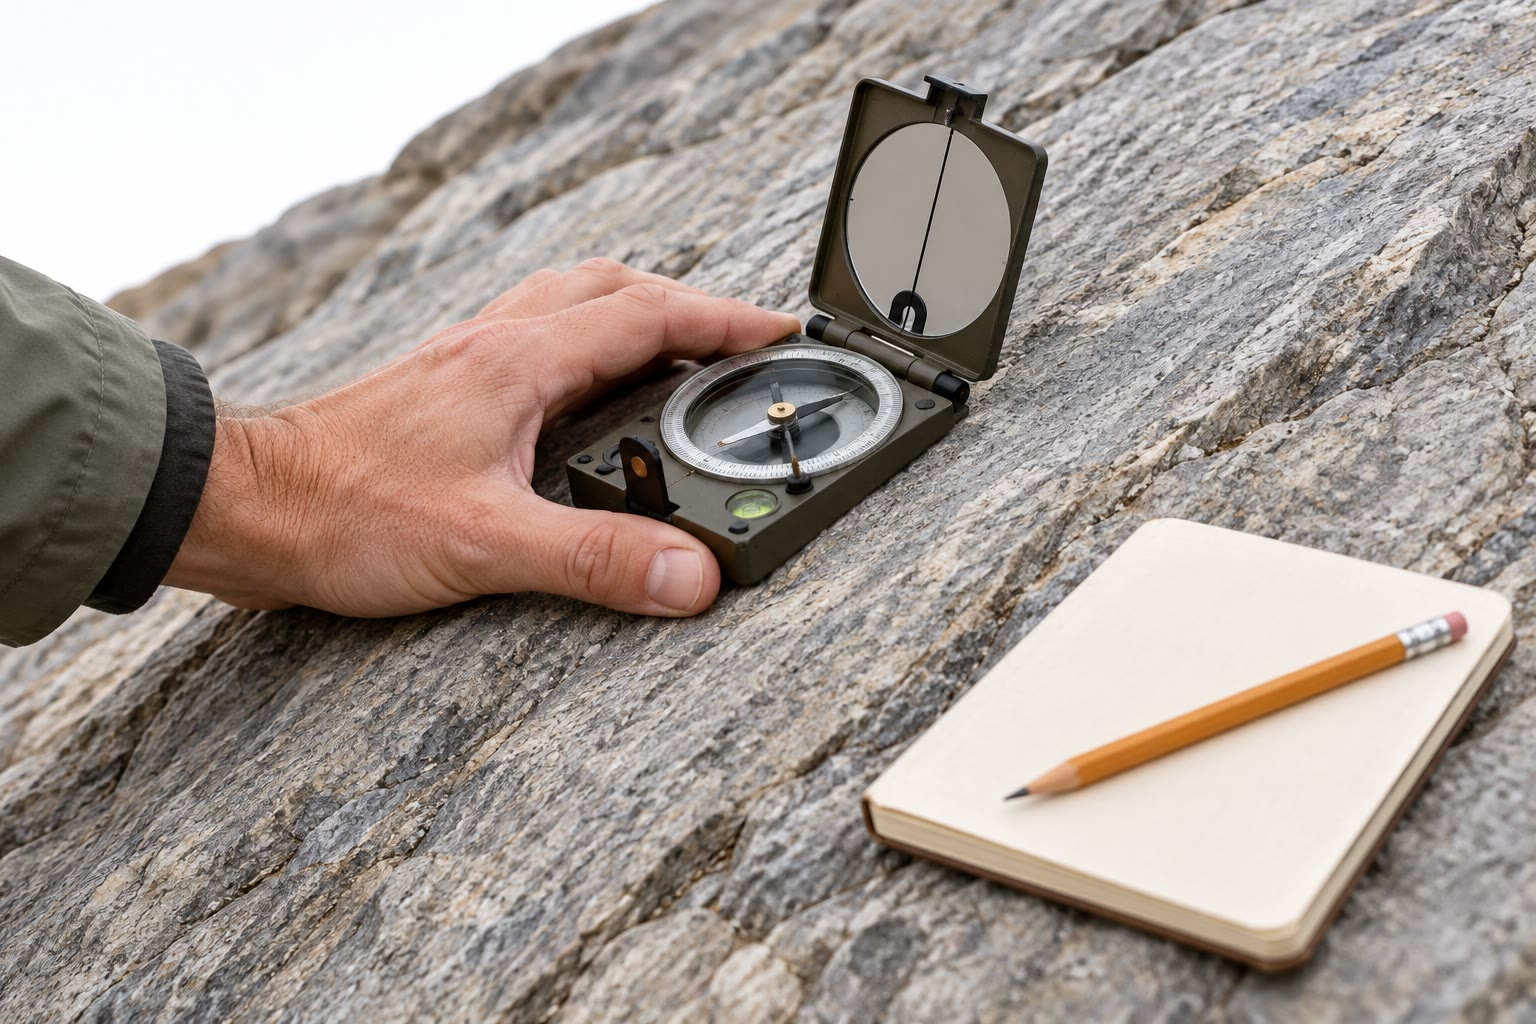
\includegraphics[width=\linewidth]{images/book5/ai/b3-compass-clinometer.jpg}

{\scriptsize Kompas-klinometer diletakkan pada permukaan batuan yang miring, dengan
buku catatan lapangan (ilustrasi buatan AI).}
\end{minipage}
\end{inthefield}

\section{Latihan}

\begin{exercise}[$\star$]\label{exo:b3:structural-analysis:1}
Tentukan tren dan penunjaman \omterm{def:b3:structural-analysis:stereo}{kutub} bidang $040/30$ (arah kemiringan,
kemiringan). Tentukan orientasi bidang yang \omterm{def:b3:structural-analysis:stereo}{kutubnya} memiliki tren \ang{315} dan penunjaman
\ang{20}.
\end{exercise}

\begin{exercise}[$\star$]\label{exo:b3:structural-analysis:2}
Sebuah garis memiliki penunjaman \ang{30}. Pada jarak berapa dari pusat, garis itu terpetakan pada
\omterm{def:b3:structural-analysis:stereo}{jaring sama sudut} dan pada jaring sama luas, keduanya dengan jari-jari \qty{10}{cm}?
\end{exercise}

\begin{exercise}[$\star$]\label{exo:b3:structural-analysis:3}
Sayap-sayap sebuah lipatan memiliki orientasi $090/30$ dan $270/30$. Hitung sudut antara
\omterm{def:b3:structural-analysis:stereo}{kutub-kutubnya} dengan hasil kali titik normal-normalnya, sudut antar-sayap,
dan kelas lipatannya.
\end{exercise}

\begin{exercise}[$\star$]\label{exo:b3:structural-analysis:4}
Sebuah sesar $090/60$ memuat goresan dengan rake \ang{-45}. Dengan vektor jurus $\vec s = (0, 1, 0)$ dan vektor
turun-kemiringan $\vec d$ bidang itu, pergeseran
dinding gantung adalah $\vec u = \cos r\,\vec s - \sin r\,\vec d$. Hitung
$\vec d$, $\vec u$, serta tren dan penunjaman pergeserannya. Beri nama sesar itu.
\end{exercise}

\begin{exercise}[$\star\star$]\label{exo:b3:structural-analysis:5}
Sayap-sayap sebuah lipatan memiliki orientasi $060/40$ dan $250/30$. Hitung
tren dan penunjaman sumbunya, serta sudut antar-sayapnya.
\end{exercise}

\begin{exercise}[$\star\star$]\label{exo:b3:structural-analysis:6}
Hitung pecahan luas jaring yang berada di dalam lingkaran garis-garis
yang penunjamannya lebih dari \ang{60}, pada jaring sama luas dan \omterm{def:b3:structural-analysis:stereo}{jaring sama sudut}, serta
pecahan arah belahan bumi bawah yang penunjamannya lebih dari \ang{60}.
Jaring mana yang sebaiknya dipakai untuk menghitung \omterm{def:b3:structural-analysis:stereo}{kutub}?
\end{exercise}

\begin{exercise}[$\star\star$]\label{exo:b3:structural-analysis:7}
Tiga \omterm{def:b3:structural-analysis:stereo}{kutub} terletak pada bidang vertikal timur--barat, masing-masing pada \ang{-20}, $0$, dan
\ang{20} dari vertikal: $\vec p = (\sin a, 0, -\cos a)$. Hitung \omterm{def:b3:structural-analysis:orientation-tensor}{tensor orientasinya},
nilai eigen dan vektor eigennya, serta \omterm{def:b3:structural-analysis:pi}{sumbu beta}. Mengapa
nilai eigen terkecilnya tepat nol?
\end{exercise}

\begin{exercise}[$\star\star$]\label{exo:b3:structural-analysis:8}
Letakkan pada diagram Flinn elipsoid $X : Y : Z = 3 : 1.5 : 1$, lalu elipsoid volume tetap
dengan $X = 1.8$ dan $Y = 1.1$. Hitung $k$ untuk
masing-masing dan beri nama regangannya.
\end{exercise}

\begin{exercise}[$\star\star$]\label{exo:b3:structural-analysis:9}
Dalam penampang yang dipotong sejajar peregangan, ooid yang awalnya bulat menjadi elips
dengan rasio sumbu $2.25$, semuanya sejajar, dan luasnya masing-masing
tidak berubah. Hitung peregangan utama dan perpanjangan sepanjang sumbu panjang. Sebelum regangan,
pusat-pusat ooid tidak pernah lebih dekat dari
\qty{0.4}{mm}: beri semi-sumbu rongga pada plot Fry.
\end{exercise}

\begin{exercise}[$\star\star\star$]\label{exo:b3:structural-analysis:10}
Pada $\theta = \ang{60}$ dari nadir, hitung peregangan sepanjang jari-jari,
$\mathrm dr/(R\,\mathrm d\theta)$, dan sepanjang lingkaran, $r/(R\sin\theta)$,
untuk kedua proyeksi. Periksa teorema pada proyeksi itu, lalu beri rasio sumbu oval
tempat jaring sama luas mengubah lingkaran kecil yang sangat kecil
di sana.
\end{exercise}

\begin{exercise}[$\star\star\star$]\label{exo:b3:structural-analysis:11}
Dalam rezim sesar geser, $\sigma_1$ mendatar menuju \ang{000},
$\sigma_3$ mendatar menuju \ang{090} dan $\sigma_2$ vertikal. Sebuah sesar vertikal
berjurus \ang{020}. Tanpa menghitung $\vec\tau$, tunjukkan bahwa pergeserannya
mendatar untuk setiap $\Phi$. Kemudian hitung $-\vec\tau$ untuk $\Phi = 0.4$ dengan
normal bidangnya $\vec n = (\cos\ang{20}, -\sin\ang{20}, 0)$ dan beri
arah pergeserannya.
\end{exercise}

\begin{exercise}[$\star\star\star$]\label{exo:b3:structural-analysis:12}
Sebuah penampang sepanjang \qty{20}{km} memotong rangkaian lipatan detasemen. Dua horizon
berjarak \qty{1.0}{km} satu sama lain berdiri di atas tingkat awalnya masing-masing dengan luas
\qty{6.0}{km^2} (bawah) dan \qty{7.5}{km^2} (atas). Hitung pemendekannya,
kedalaman detasemen di bawah horizon bawah, panjang awal penampang itu,
serta perubahan panjang relatifnya.
\end{exercise}

\section{Soal: Lipatan dan sesar di Varden Hills}

\begin{problem}[{Soal akhir pekan --- sumbu lipatan, tegangan sekumpulan sesar,
dan restorasi penampang, di wilayah rekaan}]
\label{pb:b3:structural-analysis:1}
% values: calc/ch08.py; figdata/bachelor-3/stereonet.py (data invented from region.py)
Di Varden Hills, wilayah rekaan seri ini, selimut Mesozoikum bertumpu di atas
batuan dasar sekis dan granit. Selimut itu dilipat menjadi antiklin dan sinklin tegak
dengan sayap lurus, lalu dipotong oleh sesar normal. Seorang
ahli geologi mengukur dua belas bidang perlapisan pada kedua sayap antiklin
(arah kemiringan/kemiringan, dalam derajat):

\begin{center}
\small
\begin{tabular}{l|cccccc}
\hline
sayap timur & 075/13 & 084/11 & 089/13 & 079/14 & 086/12 & 072/11 \\
sayap barat & 283/11 & 272/13 & 281/14 & 288/10 & 276/13 & 274/12 \\
\hline
\end{tabular}
\end{center}

Jumlah normal satuan ke atas dari keenam pembacaan tiap sayap ialah
$\vec S_E = (1.2583, 0.2017, 5.8604)$ dan $\vec S_W = (-1.2445, 0.1886,
5.8636)$ (timur, utara, atas). Lima sesar membawa goresan garis (arah kemiringan/kemiringan,
rake dari gelincir dinding gantung): $120/60/{-90}$ (sesar utama), $150/55/{-76}$,
$090/65/{-108}$, $200/70/{-78}$, dan $060/50/{-105}$. Sesar utama memiliki
lompatan vertikal \qty{200}{m}. Sumbu antiklin dan sinklin berjarak \qty{4}{km},
sehingga lipatan berulang setiap \qty{8}{km} dari timur ke barat.

\medskip\noindent\textbf{Bagian I --- Kutub dan sumbu beta.}
\begin{enumerate}
  \item Berikan tren dan penunjaman \omterm{def:b3:structural-analysis:stereo}{kutub} dari pembacaan $075/13$, dan
        jaraknya dari pusat jaring sama luas berjari-jari
        \qty{10}{cm}.
  \item Hitung normal satuan ke atas dari pembacaan $075/13$; periksanya
        terhadap $\vec S_E$ dari segi besarnya.
  \item Hitung orientasi rata-rata tiap sayap dari $\vec S_E$ dan $\vec S_W$,
        panjang resultan rata-rata, dan simpangan akar rerata kuadrat dari
        pembacaan terhadap rata-ratanya.
  \item Hitung $\vec S_E\times\vec S_W$, serta tren dan penunjaman
        dari \omterm{def:b3:structural-analysis:pi}{sumbu beta}.
  \item Hitung sudut antara kedua normal rata-rata, sudut antar-sayap,
        dan kelas lipatannya.
  \item Bidang aksial lipatan simetris ini memuat \omterm{def:b3:structural-analysis:pi}{sumbu beta} dan
        tegak lurus terhadap $\vec m_E - \vec m_W$, selisih normal satuan rata-rata.
        Berikan orientasinya; apakah lipatan itu tegak?
  \item Berikan orientasi sabuk-$\pi$, dan jelaskan mengapa \omterm{def:b3:structural-analysis:stereo}{kutub-kutub} terletak
        pada sabuk itu.
\end{enumerate}

\medskip\noindent\textbf{Bagian II --- Tensor orientasi.}
\omterm{def:b3:structural-analysis:orientation-tensor}{Tensor orientasi} dari kedua belas \omterm{def:b3:structural-analysis:stereo}{kutub} ialah
\[
  T = \begin{pmatrix} 0.04400 & 0.00035 & 0.00109\\ 0.00035 & 0.00144 & 0.03179\\
  0.00109 & 0.03179 & 0.95456 \end{pmatrix},
\]
dengan nilai eigen $0.95562$, $0.04400$, dan $0.00038$.
\begin{enumerate}[resume]
  \item Periksa bahwa jejak $T$ bernilai 1. Dengan $\vec b = (0.0053, -0.9994,
        0.0333)$, vektor satuan searah $\vec S_E\times\vec S_W$, hitung
        $\vec b^{\mathsf T}T\vec b$. Apa yang dikatakan hasil itu tentang $\vec b$?
  \item Hitung sudut akar rerata kuadrat antara \omterm{def:b3:structural-analysis:stereo}{kutub-kutub} dan sabuk itu.
  \item Jelaskan nilai $\lambda_2$ dari kemiringan kedua sayap.
  \item Apakah lipatan itu silindris dalam ketelitian pembacaan?
  \item Penunjaman \omterm{def:b3:structural-analysis:pi}{sumbu beta} ditentukan oleh kemiringan utara--selatan dari
        sabuk, yang tiap \omterm{def:b3:structural-analysis:stereo}{kutubnya} menyumbang dengan sebaran yang didapat pada
        pertanyaan 9. Perkirakan galat baku dari penunjaman itu.
\end{enumerate}

\medskip\noindent\textbf{Bagian III --- Paleotegangan.}
\begin{enumerate}[resume]
  \item Sesar utama itu jenis apa? Mengikuti Anderson, berikan
        arah $\sigma_1$, $\sigma_2$, dan $\sigma_3$.
  \item Tunjukkan dengan teorema arah gelincir bahwa sesar utama
        bergelincir lurus ke bawah sepanjang kemiringannya untuk setiap nilai $\Phi$. Apa
        yang dikatakannya tentang $\Phi$?
  \item Untuk sesar $150/55$, hitung $\vec n$ dan komponennya $n_1 =
        \vec n\cdot\vec e_1$ dan $n_2 = \vec n\cdot\vec e_2$, dengan $\vec e_1$
        vertikal dan $\vec e_2$ horizontal menuju \ang{030}.
  \item Gelincirnya memberikan $\vec w = \vec n\times\vec u = (0.771, 0.605, 0.198)$.
        Hitung $\Phi$.
  \item Tiga sesar kecil lainnya memberikan $\Phi = 0.294$, $0.301$, dan
        $0.306$. Berikan rata-rata, dan jelaskan dari mana sebarannya berasal.
  \item Apa yang dikatakan $\Phi = 0.3$ tentang $\sigma_2$?
  \item Hitung sumbu P dan T dari sesar utama (pada \ang{45} dari
        bidang, dalam bidang kemiringannya), dan bandingkan dengan $\sigma_1$ dan
        $\sigma_3$.
\end{enumerate}

\medskip\noindent\textbf{Bagian IV --- Merestorasi penampang timur--barat.}
\begin{enumerate}[resume]
  \item Hitung kemiringan semu sayap timur, $080.9/12.3$, pada
        penampang timur--barat.
  \item Dengan sayap pada \ang{12} di penampang, hitung panjang hasil restorasi
        satu gelombang lipatan, pemendekannya, dan perubahan
        panjang relatifnya.
  \item Hitung tinggi puncak antiklin di atas sinklin dan
        luas kelebihan satu panjang gelombang, dengan anggapan bahwa sinklin
        tetap pada tingkat awalnya.
  \item Hitung kedalaman detasemen di bawah lapisan terlipat. Dapatkah
        lipatan itu berdetasemen pada dasar selimut, beberapa ratus meter
        di bawah permukaan?
  \item Hitung lompatan horizontal dan gelincir sesar utama pada
        penampang sepanjang \ang{120}.
  \item Pada penampang timur--barat, hitung kemiringan semu sesar dan
        lompatan horizontal semunya. Penampang mana yang harus direstorasi?
  \item Dalam urutan apa sesar dan lipatan direstorasi, dan di mana
        \omterm{def:b3:structural-analysis:restoration}{garis pasak} diletakkan?
  \item Berapa penunjaman sumbu lipatan Varden yang diperoleh dari kedua belas
        pembacaan?
\end{enumerate}
\end{problem}
